% sets default font to Arial
\renewcommand{\rmdefault}{phv} % Arial
\renewcommand{\sfdefault}{phv} % Arial\\

%font size, document type and paper size
\documentclass[11pt,a4paper]{article}

\title{CMEE Miniproject}
\date{05 March 2019}
\author{Katherine Bickerton}

\usepackage[left=2cm,right=2cm,top=2cm,bottom=2cm]{geometry} % set page margins
\usepackage{lineno} % select specific line spacing
\linespread{2}
\usepackage{pgfplotstable} % generate tables
\usepackage{graphicx} % inserting graphics
\usepackage{float} % positioning images
\usepackage{subcaption} % allow multiple figures
\usepackage{titlesec} % generate title page
\titleformat*{\section}{\large\bfseries}
\titleformat*{\subsection}{\normalsize\bfseries}
\usepackage{amsmath} % equation formatting
\usepackage{amssymb} % symbols for equations
\usepackage[round]{natbib} % generate biblography
\bibliographystyle{unsrtnat} % specific style of bibliography

\begin{document}
	
	\begin{titlepage}
		\centering
		\topskip4cm
		{\Large
			\vskip4cm
			CMEE MiniProject:~\\
			\vskip1cm
			You are what you eat; Model optimisation for predicting predator size from prey size and associated abiotic factors, in global marine systems.
		}    
		\vskip2cm	
		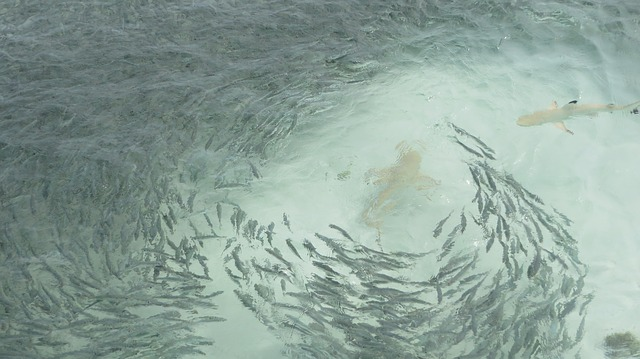
\includegraphics[width = 15cm]{predprey.jpg}
		\vskip2cm	
		Katherine Bickerton, \textit{Imperial College, London}\\
		\vskip1cm		
		Word Count = [2597]
		\vspace*{\fill}
		\vspace*{\fill}
	\end{titlepage}
	
	
	\Large \noindent You are what you eat; Model optimisation for predicting predator size from prey size and associated abiotic factors, in global marine systems.
	\linenumbers
	
	\normalsize	
	\section{Abstract}
	
	\par \noindent Marine systems are one of the most difficult to monitor on the planet and one of the most at risk. Those at higher trophic levels are often the most at risk due to dependence on the stability of the rest of the food web. In this study, I aim to compare linear regression, generalised additive (GAM) and generalised linear mixed effects (GLMM) models for predicting predator size, based upon prey size, feeding interaction, habitat, temperature and depth. The optimal model was a generalised additive model (GAM), with prey mass, temperature and depth as explanatory variables. Feeding interaction was also found to have an effect using GLMM, but violated the assumptions of GAM, therefore could not be included in the optimal model. These findings implies that predator size could be predicted from prey size and abiotic factors, which are less labour intensive to collect and could improve efficiency of conservation research.
	
	\section{Introduction}
	
	\par \noindent With ever increasing risks to biodiversity \citep{Kerr1995}, and the close proximity of a sixth mass extinction extinction event \citep{Barnosky2011}, understanding the dynamics of ecological systems is increasingly important. One of the main threats to biodiversity is overexploitation, where many populations have been reduced to an unsustainable level. This is especially true of marine systems where, despite regulations, approximately 63\% of fish stocks are below a the threshold population size required to persist \citep{Heithaus2008}.
	
	\par \noindent ~\\ Population data is particularly difficult to collect in marine systems, especially on pelagic organisms in deep oceans, often restricting data collection to shallow coastal areas. One means of supplementing information in data poor systems is to construct predictive models from existing data and extrapolate with a variety of parameters \citep{Levins1966}. This method can also aid in targeting studies to test likely models and aid in mitigation against overexploitation.
	
	\par \noindent ~\\ One classical model within ecosystem dynamics is that between predators and prey \citep{Freedman1983}. Information regarding predator and prey physiology and consumption is some of the most easily available in marine systems. The most common method is stomach contents analysis of organisms caught as by-catch or stranded \citep{Turesson2002}. This allows understanding of the position of each species within the food chain, and which prey sources are most important to or most threatened by specific predators. 
	
	\par \noindent ~\\ This study uses an existing dataset of marine predators, both in coastal and pelagic zones to construct a model that could be used to predict predator size based upon available prey. The main aim is to investigate the relationship between predator mass and  prey mass, on a global scale, across a range of habitats, temperatures and depths. As opposed to defining a typical "null hypothesis", this study is considering several different models for predator mass, based on the above factors, and will select and interpret the optimal model for the system.
	
	\section{Methods}
	
	\subsection{Data Compilation}
	
	\par \noindent The data used for this was complied by Barnes et al, 2008, and comprises 19,625 records of 57 different marine predator species, from 27 locations globally, and 18 studies \citep{Barnes2008}. The dataset included predator species, masses and lengths of predators and prey, habitat, location, type of feeding interaction, depth, mean annual air temperature and mean annual precipitation, for each predation record.
	
	\par \noindent ~\\As this study aimed to examine relationship between predator and prey sizes, I chose one dimension, mass, as the measure of size, and excluded length as the two variables would violate the assumption of independence. The mean average of predator and prey masses, temperature and depth for each predator species were calculated. For the categorical variables, habitat and feeding interaction, the most common for each predator species was selected. Habitats were sorted into coastal and pelagic, dependent on the definitions of the habitats mentioned in each study. Feeding interactions were classified into either piscivorous (feeding only on fish), predacious (generalist predators, though diet may include fish), and planktivorous (feeding only on plankton), as defined by Barnes et al, 2008. A new data frame was compiled containing the averages calculated for each species, then used in model fitting.
	
	\subsection{Model Building and Fitting}
	
	\par \noindent I chose to compare three different types of model: a linear regression model, a generalised additive model (GAM) and a generalised linear mixed effects model (GLMM). The response variable, predator mass, did not have a linear distribution, therefore it was log transformed for use in the linear models, and as the response variable must be consistent for models to be comparable, predator mass was also log transformed for the GAM.
	
	\par \noindent ~\\When building the models, I started with the assumption that predator mass would be a function of the average mass of prey species. Additional explanatory variables were also considered and selected for in each model, dependent on whether they improved model fit, described below. The additional variables considered were: feeding interaction, habitat, depth and temperature. For each model, combinations of the explanatory variable were tested and the Akaike Information Criterion (AIC) calculated for each model, then compared to give the best fit to the data. The optimal models from each type of model were then compared, again using AIC, to find the model that overall best described the data. The linear regression model comparison was carried out using the "step" function in R, however no equivalent function was available for GAMs and GLMMs, so comparisons were carried out manually using anova tests and AIC to systematically reject variables which decreased the fit of the model. 
	
	\par \noindent ~\\ \textbf{Model 1: Linear Regression Model -}  The linear regression model for predator mass was defined as below, where m = mass in grams and $\epsilon$ is the error not explained by the explanatory variable. 
	
		\begin{equation*}
			m_{pred} \sim m_{prey} + \epsilon
		\end{equation*}
	
	\noindent ~\\ Linear regression models assume that the data is linear, therefore predator mass, prey mass and mean depth were log transformed. It also assumes collinearity and independence \citep{Zuur2009}, therefore any explanatory variables that could interact must be removed. Due to this, habitat and feeding interaction were removed from the model as they correlated with depth and prey mass respectively. Finally, normally distributed variables are required, which occurred when the data was log transformed.
	
	\par \noindent ~\\ \textbf{Model 2: GAM -} The general additive model uses a smoothing function on each explanatory variable, to map each individuals fit to the response variable, and uses a Gaussian distribution as the variables used are continuous. The equation takes the following form, where m = mass, f denotes the smoothing function, x$_{n}$ denote the explanatory variable and $\epsilon$ is error not explained by the variables.
	
		\begin{equation*}
			m_{pred} \sim f(x_{1}) + f(x_{2}) + ... + f(x_{n}) + \epsilon
		\end{equation*}
		
	\noindent ~\\ The assumptions for GAM also require independence therefore habitat and feeding interaction were also excluded from the GAM models. Log transforms were not required for the model, as GAMs do not require linear variables \citep{Zuur2009}, however log transformed models were compared as they were used in the previous model.
	
	\par \noindent ~\\ \textbf{Model 3: GLMM -} Mixed models give the ability to account for non-independence of variables by adding them as random effects, meaning they effect the data but not predictably \citep{Zuur2009}. The following equation gives the general model for the GLMM, where m = mass, subscripts indicate fixed and random variables, d = mean depth, h = habitat, i = feeding interaction and $\epsilon$ accounts for any other error.
	
		\begin{equation*}
			m_{pred} \sim m_{prey - fixed} + d_{fixed} + h_{random} + i_{random} + \epsilon
		\end{equation*}
		
	\par \noindent ~\\ As a type of linear model, prey mass and depth were both log transformed to give a linear distribution. Additionally collinearity and independence are also assumptions of GLMMs unless the non-independent factors are accounted for as random effects, allowing the inclusion of habitat and feeding interactions in this model. 


	\subsection{Computing Languages}
	
	\par \noindent Python version 3.5.2 \citep{PythonCoreTeam2018} was used to manipulate the raw data into the data frame used for model building, as the pandas package \citep{mckinney-proc-scipy-2010} is fast and efficient at manipulating and building data frames and csv files.
	\par \noindent ~\\R version 3.4.4 \citep{RCoreTeam2018} was used for model fitting, selection and plotting models. R was most appropriate for this due to the wealth of packages available for model fitting and plotting. The package mgcv \citep{Wood2011} fits GAM models and allows plots equivalent to the residual plots that can be produced for linear models. The lme4 package \citep{Bates2015} fits linear mixed effects models and gives information about the significance of each different factor. R also has an inbuilt function to calculate the Akaike Information Criterion which was used to select the optimal model. Finally, the ggplot2 \citep{Wickham2016} package was used to generate plots used in this report (specified in figure legend when used).
	
	\par \noindent ~\\Shell scripts in bash were used to compile the \LaTeX \ document into a pdf format with references from the associated BibTeX file and to run the final project, as bash has inbuilt commands to run R and Python script files.
	
	\section{Results}
	
	\subsection{Model 1: Linear Regression Model}
	
	\par \noindent Initially the linear regression model tested contained the three independent explanatory variables: prey mass, depth and temperature. To fulfil the assumption of linearity, prey mass and depth were both log transformed  (note that predator mass is log transformed for all models), and a comparison using AIC was made between the fit of the model with and without log transforms (AIC$_{notlogged}$ = 343.8, AIC$_{logged}$ = 236.1). The smaller AIC value of the log transformed model indicated that it better fitted the data and the large difference between the values shows a significantly different fit.
	
	\par \noindent ~\\ Each variable in the model was then tested using the step function in R, which removed the least significant variable in the model then refitted it to the data until the optimal model was found. This model only contained one significant explanatory variable, prey mass (linear regression: R$^2$ = 0.90, F$_{1,55}$ = 496.3, p $<$ 0.001). The R$^2$ value for this model was high and positive meaning 90\% of the variation in predator mass could be explained by prey mass. Figure \ref{fig:linmod}a indicates the fit of the regression model (shown by a black line) to the data. The coefficients of the regression line were extracted from the model to give an overall equation of:
	
	\begin{equation*}
		log(m_{pred}) = 5.41 + 0.761log(m_{prey})
	\end{equation*}
	
	\par \noindent ~\\ Where m = mass in grams, therefore when predator mass increases with prey mass.
	
	\begin{figure}[H]
		\centering %centre figure
		% set line width manually
		\begin{subfigure}[t]{0.45\linewidth}
			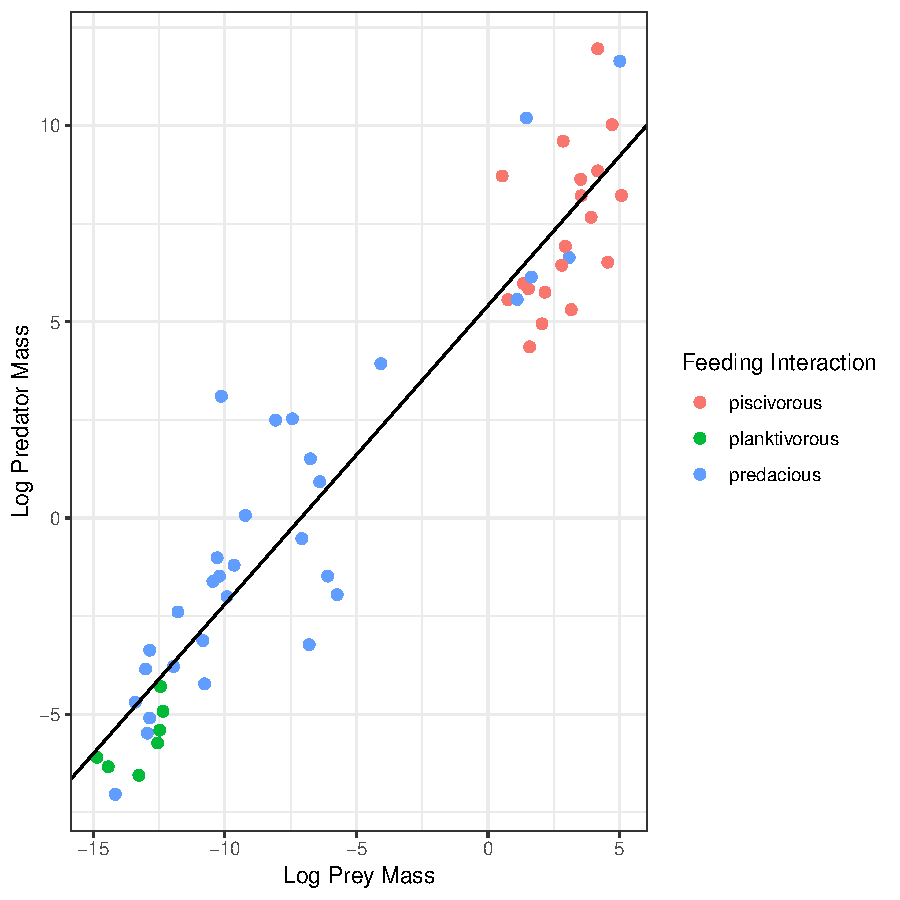
\includegraphics[width=\linewidth]{../Results/lin_mod_feeding.pdf}
			\caption{}
		\end{subfigure}
		\begin{subfigure}[t]{0.45\linewidth}
			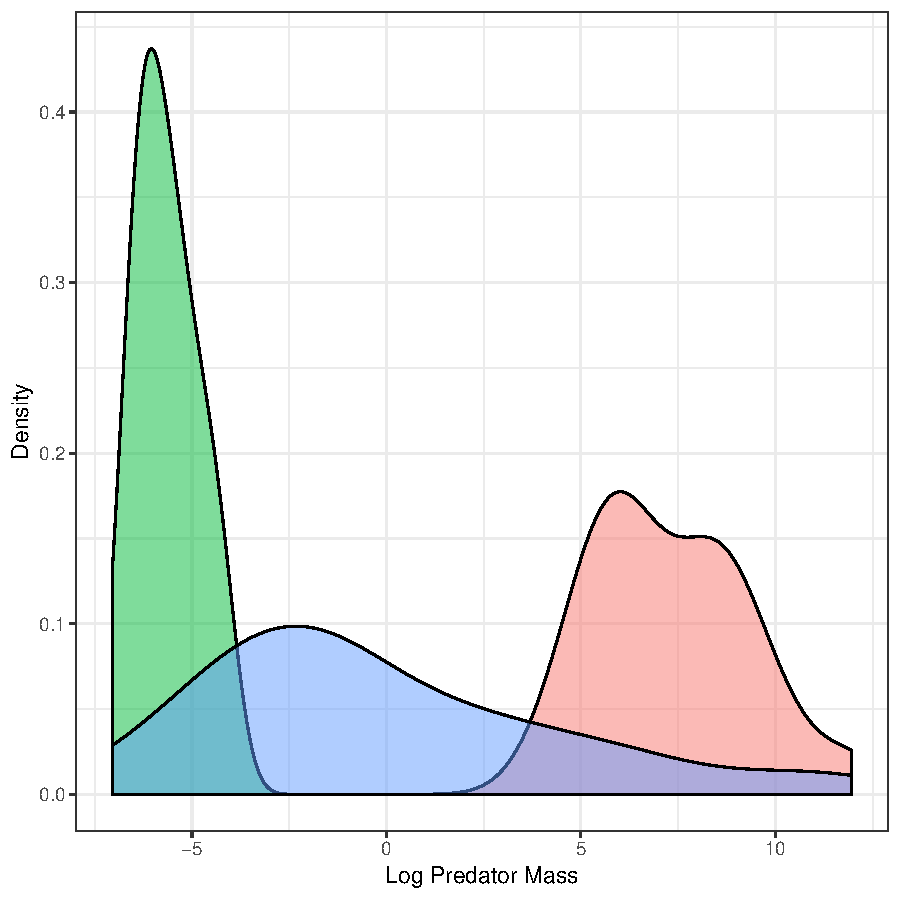
\includegraphics[width=\linewidth]{../Results/density_feeding.pdf}
			\caption{}
		\end{subfigure}
		\caption{(a) Mean average mass of 57 predator species as a function of mean average mass of prey, both log transformed. The black line represents the linear regression model: $log(m_{pred}) = 5.41 + 0.761log(m_{prey})$, colours represent the three feeding interactions, piscivorous (red,n=19), predacious (blue, n=31) and planktivorous (green, n=7). (b) Density plot of log transformed mean average predator masses by feeding interaction, colours same as (a).}
		\label{fig:linmod}
	\end{figure}
	
	\par \noindent ~\\ Although feeding interaction was not accounted for in the linear regression model, due to possible correlation with prey size, I split Figure \ref{fig:linmod}a by feeding interaction and there appears to be strong grouping, with larger predators tending to be piscivorous and smaller to be planktivorous, with generalised predation more broadly spread. This relationship is further explored in Figure \ref{fig:linmod}b, a density plot of each feeding interaction against predator mass, which reiterates this relationship. Planktivorous species also appear to be confined to a small range of predator masses whereas piscivorous cover a broader range of predator masses. This is explained further in the linear mixed model section.
		
	\subsection{Model 2: Generalised Additive Model (GAM)}
	
	\par \noindent The initial GAM, as with the linear regression model, included all independent explanatory variables, however there is no equivalent of the step function available for GAMs so models fits were tested manually. In each step, the least significant factor was removed, and model refitted, then compared to the previous model. Log transforms were also tested in the same way. The final model with the best fit to the data contained all three explanatory variables, but only prey mass was log transformed:
	
	\begin{equation*}
		log(m_{pred}) \sim f(log(m_{prey})) + f(temp) + f(depth) + \epsilon
	\end{equation*}
	
	\par \noindent ~\\ Where m = mass in gramms, $\epsilon$ indicates error not accounted for by the explanatory variables, and all variables are averaged. Figure \ref{fig:gammod} shows the relationship between each of the smoothed variables and predator mass. Figure\ref{fig:gammod}top shows predator mass increased with prey mass, as seen in the linear regression model. Figure \ref{fig:gammod}middle  shows a more complex relationship with the smallest predators found at lower temperatures, then medium to larger predators varying within a similar range of temperatures. Figure \ref{fig:gammod}bottom shows another linear relationship where larger predators are found at higher depths, whereas small predators tend to stay in shallower areas.
	 
	
	\begin{figure}[H]
		\centering %centre figure
		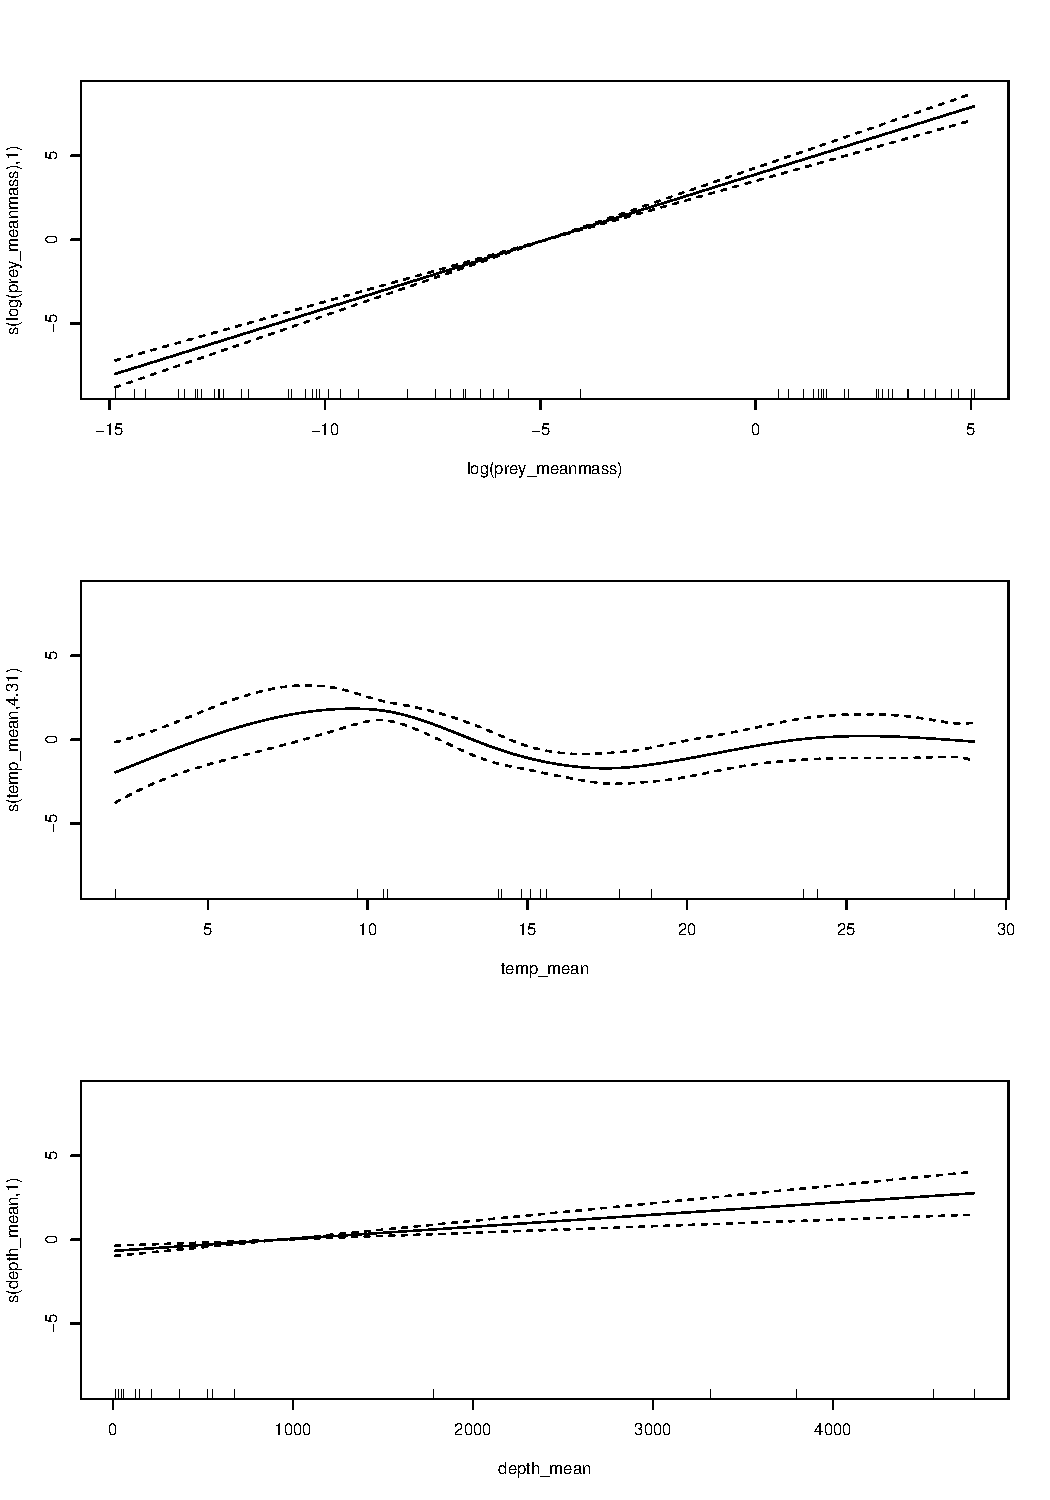
\includegraphics[width=0.8\linewidth]{../Results/gam_mod_plot.pdf}
		\caption{Smoothed functions of the explanatory variables used in the GAM model, where dotted lines give standard error and average predator mass is log transformed, n=57. Top: predator mass increases linearly with log transformed prey mass, middle: temperature fluctuates with predator mass change, indicating no clear relationship, bottom: predator mass increase linearly with depth.}
		\label{fig:gammod}
	\end{figure}	

	\subsection{Model 3: Linear Mixed Effects Model (GLMM)}	
	
	\par \noindent As with the first two models, I started the GLMM model with the maximum explanatory variables, including habitat and feeding interaction as random effects which allows for their lack of independence. I then compared the models manually, excluding the least significant factor and comparing the fit of the new models using analysis of variance (ANOVA) as GLMMs are a type of linear model. The AIC values calculated gave the best fitting model as:
	
	\begin{equation*}
		log(m_{pred}) \sim log(m_{prey}) + feeding_{random} + \epsilon
	\end{equation*}
	
	\par \noindent Where m = mass in grams, feeding interaction is included as a random effect and epsilon indicates variance not explained by the other variables. This model produced a very similar relationship to the linear regression model, however also explains the grouped feeding interactions observed in Figure \ref{fig:linmod}.
	
	\subsection{Model Selection}
	
	\par \noindent Once optimal models were chosen for each type of model, the AIC values were compared, with the linear regression model giving an AIC = 232.5, GAM AIC = 200.4 and GLMM AIC = 239.0, therefore the GAM has the best fit. Additionally, Figure \ref{fig:resid} shows the residual plots for each of the final models, and GAM has the narrowest range of residuals and most even spread compared to the other models, further supporting that it is the most appropriate model for the data.
	
	\begin{figure}[H]
		\centering %centre figure
		% set line width manually
		\begin{subfigure}[t]{0.6\linewidth}
			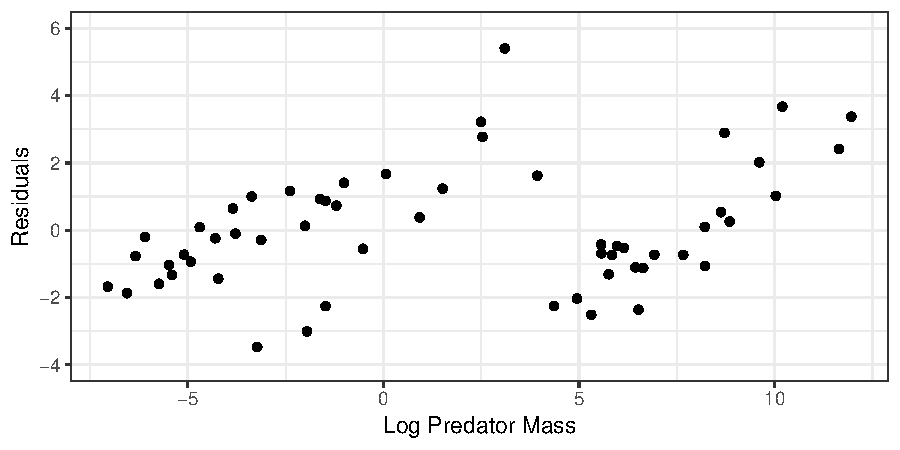
\includegraphics[width=\linewidth]{../Results/lin_mod_resid.pdf}
			\caption{}
		\end{subfigure}
		\begin{subfigure}[t]{0.6\linewidth}
			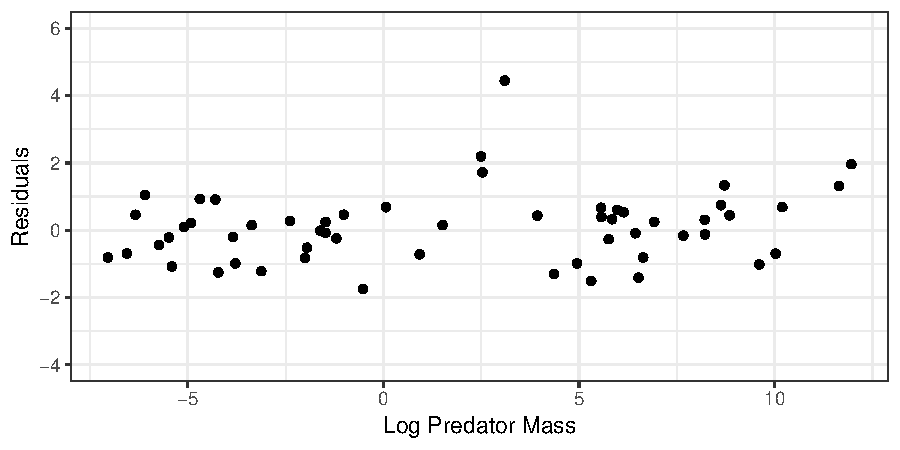
\includegraphics[width=\linewidth]{../Results/gam_mod_resid.pdf}
			\caption{}
		\end{subfigure}
		\begin{subfigure}[t]{0.6\linewidth}
			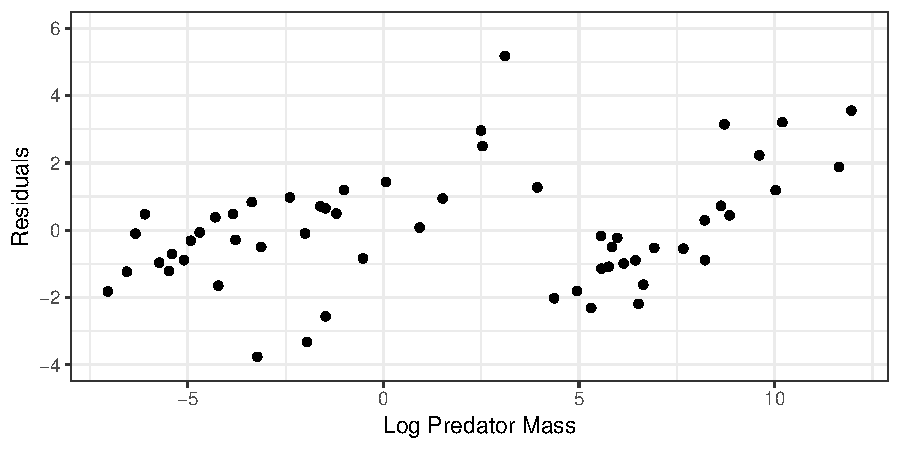
\includegraphics[width=\linewidth]{../Results/glmm_mod_resid.pdf}
			\caption{}
		\end{subfigure}
		\caption{}
		\label{fig:resid}
	\end{figure}
	
	
	\section{Discussion}
	
	\par \noindent This study aimed to find an optimum model with which to predict predator mass, based upon a range of potential factors. Three types of model were tested: linear regression, generalised additive (GAM) and generalised linear mixed effects (GLMM), and the optimal model was found using GAM method. This model indicated that predator mass was a function of average prey mass, annual air temperature at the location and average depth at which the prey species was found. Predator mass (averaged and log tranformed) had a positive linear relationship with prey mass, therefore as prey mass increased, so did predator mass. Additionally, predator mass also increased with depth and varied with temperature fluctuations.
	
	\par \noindent ~\\ Many marine predators, especially those of larger mass, tend to have large home ranges and encounter a wide variety of prey \citep{Costa2016}. This makes them particularly difficult to monitor, whereas smaller species are often more localised, therefore easily monitored. The model generated could be useful in locations where potential prey species are present, as expected size of predator species could be predicted. This could also highlight those areas where predators are absent despite prey availability. Furthermore, species at higher trophic levels tend to be more vulnerable to disturbance as their persistence depends on an entire chain of species, as opposed to one producer \citep{Purvis2000}, so having a means to predict their presence, or lack of, could aid monitoring groups globally.
	
	\par \noindent ~\\ In the optimal GLMM, the factor of feeding interaction was present, and relatively distinct clusters for piscivorous and planktivorous species were shown in \ref{fig:linmod}. However, this variable was not included in the final model as it was unlikely to be independent of prey mass, and GAMs do not allow for random effects. Despite this, it is likely that feeding interaction does effect predator mass. This could be accounted for by generalised additive mixed effect models \citep{Zuur2009}, which combine the inclusion of random effects with a GAM, and would be the next logical step from this study.
	
	\par \noindent ~\\ Another important assumption of this study, was that density of predators or prey had no affect on predator mass or was constant. This may oversimplify the system as, for example, many whale species feed on plankton however the density of plankton allow a much higher body mass and many piscivorous fish species have been observed increasing predation when only smaller prey species are available \citep{Vezina1985}. This contradicts the findings in this study that indicated planktivorous predators had some of the lowest body masses. Therefore, another area for further study would be to include a factor for density into the model.
	
	\subsection{Conclusion}	
	
	\par \noindent Overall, this study showed that the assumptions of models can have a marked effect on which explanatory variables are selected during optimisation. For marine predator prey systems, GAM were found to have the best fit to the data, and the function of mixed effects models to include random effects also showed interactions that may have otherwise been missed. To further this study, models combining these two types of model are advised, especially if used in predictions for conservation.
	
	\bibliography{miniproject}
	
	
\end{document}
